\documentclass[a4paper,11pt,fleqn,dvipsnames,twoside,openany]{memoir} 	% Openright aabner kapitler paa hoejresider (openany begge)

%\documentclass[a4paper,11pt,fleqn,dvipsnames,twoside,openright]{memoir} 	% Openright aabner kapitler paa hoejresider (openany begge)

%%%% PACKAGES %%%%

% ¤¤ Oversaettelse og tegnsaetning ¤¤ %
\usepackage[utf8]{inputenc}					% Input-indkodning af tegnsaet (UTF8)
\usepackage[danish]{babel}					% Dokumentets sprog
\usepackage[T1]{fontenc}					% Output-indkodning af tegnsaet (T1)
\usepackage{ragged2e,anyfontsize}			% Justering af elementer
\usepackage{fixltx2e}						% Retter forskellige fejl i LaTeX-kernen
%\usepackage[utf8]{inputenc}
																			
% ¤¤ Figurer og tabeller (floats) ¤¤ %
\usepackage{graphicx} 						% Haandtering af eksterne billeder (JPG, PNG, EPS, PDF)
\graphicspath{ {billeder/} }

\usepackage{sidecap}
%\usepackage{eso-pic}						% Tilfoej billedekommandoer paa hver side
\usepackage{wrapfig}						% Indsaettelse af figurer omsvoebt af tekst. \begin{wrapfigure}{Placering}{Stoerrelse}
\usepackage{multirow}                		% Fletning af raekker og kolonner (\multicolumn og \multirow)
\usepackage{multicol}         	        	% Muliggoer output i spalter
\usepackage{rotating}						% Rotation af tekst med \begin{sideways}...\end{sideways}
\usepackage{colortbl} 						% Farver i tabeller (fx \columncolor og \rowcolor)
\usepackage{xcolor}							% Definer farver med \definecolor. Se mere: http://en.wikibooks.org/wiki/LaTeX/Colors
\usepackage{flafter}						% Soerger for at floats ikke optraeder i teksten foer deres reference
\let\newfloat\relax 						% Justering mellem float-pakken og memoir
\usepackage{float}							% Muliggoer eksakt placering af floats, f.eks. \begin{figure}[H]
\usepackage{wrapfig}

% ¤¤ Matematik mm. ¤¤
\usepackage{amsmath,amssymb,stmaryrd} 		% Avancerede matematik-udvidelser
\usepackage{mathtools}						% Andre matematik- og tegnudvidelser
\usepackage{textcomp}                 		% Symbol-udvidelser (f.eks. promille-tegn med \textperthousand )
\usepackage{rsphrase}						% Kemi-pakke til RS-saetninger, f.eks. \rsphrase{R1}
\usepackage[version=3]{mhchem} 				% Kemi-pakke til flot og let notation af formler, f.eks. \ce{Fe2O3}
\usepackage{siunitx}						% Flot og konsistent praesentation af tal og enheder med \si{enhed} og \SI{tal}{enhed}
\sisetup{output-decimal-marker = {,}}		% Opsaetning af \SI (DE for komma som decimalseparator) 

% ¤¤ Referencer og kilder ¤¤ %
\usepackage[danish]{varioref}				% Muliggoer bl.a. krydshenvisninger med sidetal (\vref)
\usepackage{natbib}							% Udvidelse med naturvidenskabelige citationsmodeller
%\usepackage{xr}							% Referencer til eksternt dokument med \externaldocument{<NAVN>}
%\usepackage{glossaries}					% Terminologi- eller symbolliste (se mere i Daleifs Latex-bog)

% ¤¤ Misc. ¤¤ %
\usepackage{listings}						% Placer kildekode i dokumentet med \begin{lstlisting}...\end{lstlisting}
\usepackage{lipsum}							% Dummy text \lipsum[..]
\usepackage[shortlabels]{enumitem}			% Muliggoer enkelt konfiguration af lister
\usepackage{pdfpages}						% Goer det muligt at inkludere pdf-dokumenter med kommandoen \includepdf[pages={x-y}]{fil.pdf}	
\pdfoptionpdfminorversion=6					% Muliggoer inkludering af pdf dokumenter, af version 1.6 og hoejere
\pretolerance=2500 							% Justering af afstand mellem ord (hoejt tal, mindre orddeling og mere luft mellem ord)

% Kommentarer og rettelser med \fxnote. Med 'final' i stedet for 'draft' udloeser hver note en error i den faerdige rapport.
\usepackage[footnote,draft,danish,silent,nomargin]{fixme}		


%%%% CUSTOM SETTINGS %%%%

% ¤¤ Marginer ¤¤ %
%\setlrmarginsandblock{3.5cm}{2.5cm}{*}
\setlrmarginsandblock{2.5cm}{2.5cm}{*} %\setlrmarginsandblock{Indbinding}{Kant}{Ratio}
\setulmarginsandblock{2.5cm}{2.5cm}{*}		% \setulmarginsandblock{Top}{Bund}{Ratio}
\checkandfixthelayout 						% Oversaetter vaerdier til brug for andre pakker

%	¤¤ Afsnitsformatering ¤¤ %
\setlength{\parindent}{0mm}           		% Stoerrelse af indryk
\setlength{\parskip}{3mm}          			% Afstand mellem afsnit ved brug af double Enter
\linespread{1,1}							% Linie afstand

% ¤¤ Litteraturlisten ¤¤ %
\bibpunct[,]{[}{]}{;}{a}{,}{,} 				% Definerer de 6 parametre ved Harvard henvisning (bl.a. parantestype og seperatortegn)
\bibliographystyle{bibtex/harvard}			% Udseende af litteraturlisten.

% ¤¤ Indholdsfortegnelse ¤¤ %
\setsecnumdepth{subsection}		 			% Dybden af nummerede overkrifter (part/chapter/section/subsection)
\maxsecnumdepth{subsection}					% Dokumentklassens graense for nummereringsdybde
\settocdepth{subsection} 					% Dybden af indholdsfortegnelsen

% ¤¤ Lister ¤¤ %
\setlist{
  topsep=0pt,								% Vertikal afstand mellem tekst og listen
  itemsep=-1ex,								% Vertikal afstand mellem items
} 

% ¤¤ Visuelle referencer ¤¤ %
\usepackage[colorlinks]{hyperref}			% Danner klikbare referencer (hyperlinks) i dokumentet.
\hypersetup{colorlinks = true,				% Opsaetning af farvede hyperlinks (interne links, citeringer og URL)
    linkcolor = black,
    citecolor = black,
    urlcolor = black
}

% ¤¤ Opsaetning af figur- og tabeltekst ¤¤ %
\captionnamefont{\small\bfseries\itshape}	% Opsaetning af tekstdelen ('Figur' eller 'Tabel')
\captiontitlefont{\small}					% Opsaetning af nummerering
\captiondelim{. }							% Seperator mellem nummerering og figurtekst
\hangcaption								% Venstrejusterer flere-liniers figurtekst under hinanden
\captionwidth{\linewidth}					% Bredden af figurteksten
\setlength{\belowcaptionskip}{0pt}			% Afstand under figurteksten
		
% ¤¤ Opsaetning af listings ¤¤ %

\definecolor{commentGreen}{RGB}{34,139,24}
\definecolor{stringPurple}{RGB}{208,76,239}

\lstset{language=Matlab,					% Sprog
	basicstyle=\ttfamily\scriptsize,		% Opsaetning af teksten
	keywords={for,if,while,else,elseif,		% Noegleord at fremhaeve
			  end,break,return,case,
			  switch,function},
	keywordstyle=\color{blue},				% Opsaetning af noegleord
	commentstyle=\color{commentGreen},		% Opsaetning af kommentarer
	stringstyle=\color{stringPurple},		% Opsaetning af strenge
	showstringspaces=false,					% Mellemrum i strenge enten vist eller blanke
	numbers=left, numberstyle=\tiny,		% Linjenumre
	extendedchars=true, 					% Tillader specielle karakterer
	columns=flexible,						% Kolonnejustering
	breaklines, breakatwhitespace=true,		% Bryd lange linjer
}

% ¤¤ Navngivning ¤¤ %
\addto\captionsdanish{
	\renewcommand\appendixname{Appendiks}
	\renewcommand\contentsname{Indholdsfortegnelse}	
	\renewcommand\appendixpagename{Appendiks}
	\renewcommand\appendixtocname{Appendiks}
	\renewcommand\cftchaptername{\chaptername~}				% Skriver "Kapitel" foran kapitlerne i indholdsfortegnelsen
	\renewcommand\cftappendixname{\appendixname~}			% Skriver "Appendiks" foran appendiks i indholdsfortegnelsen
}

% ¤¤ Kapiteludssende ¤¤ %
\definecolor{numbercolor}{gray}{0.7}		% Definerer en farve til brug til kapiteludseende
\newif\ifchapternonum

\makechapterstyle{jenor}{					% Definerer kapiteludseende frem til ...
  \renewcommand\beforechapskip{0pt}
  \renewcommand\printchaptername{}
  \renewcommand\printchapternum{}
  \renewcommand\printchapternonum{\chapternonumtrue}
  \renewcommand\chaptitlefont{\fontfamily{pbk}\fontseries{db}\fontshape{n}\fontsize{25}{35}\selectfont\raggedleft}
  \renewcommand\chapnumfont{\fontfamily{pbk}\fontseries{m}\fontshape{n}\fontsize{1in}{0in}\selectfont\color{numbercolor}}
  \renewcommand\printchaptertitle[1]{%
    \noindent
    \ifchapternonum
    \begin{tabularx}{\textwidth}{X}
    {\let\\\newline\chaptitlefont ##1\par} 
    \end{tabularx}
    \par\vskip-2.5mm\hrule
    \else
    \begin{tabularx}{\textwidth}{Xl}
    {\parbox[b]{\linewidth}{\chaptitlefont ##1}} & \raisebox{-15pt}{\chapnumfont \thechapter}
    \end{tabularx}
    \par\vskip2mm\hrule
    \fi
  }
}											% ... her

\chapterstyle{jenor}						% Valg af kapiteludseende - Google 'memoir chapter styles' for alternativer

% ¤¤ Sidehoved ¤¤ %

\makepagestyle{AAU}							% Definerer sidehoved og sidefod udseende frem til ...
\makepsmarks{AAU}{%
	\createmark{chapter}{left}{shownumber}{}{. \ }
	\createmark{section}{right}{shownumber}{}{. \ }
	\createplainmark{toc}{both}{\contentsname}
	\createplainmark{lof}{both}{\listfigurename}
	\createplainmark{lot}{both}{\listtablename}
	\createplainmark{bib}{both}{\bibname}
	\createplainmark{index}{both}{\indexname}
	\createplainmark{glossary}{both}{\glossaryname}
}
\nouppercaseheads											% Ingen Caps oenskes

\makeevenhead{AAU}{Gruppe A401}{}{Aalborg Universitet}
%\makeevenhead{AAU}{Gruppe A401}{}{\leftmark}				% Definerer lige siders sidehoved (\makeevenhead{Navn}{Venstre}{Center}{Hoejre})
\makeoddhead{AAU}{Gruppe A401}{}{Aalborg Universitet}
%\makeoddhead{AAU}{\rightmark}{}{Aalborg Universitet}		% Definerer ulige siders sidehoved (\makeoddhead{Navn}{Venstre}{Center}{Hoejre})
\makeevenfoot{AAU}{}{}{\thepage}{}{}							% Definerer lige siders sidefod (\makeevenfoot{Navn}{Venstre}{Center}{Hoejre})
\makeoddfoot{AAU}{}{}{\thepage}								% Definerer ulige siders sidefod (\makeoddfoot{Navn}{Venstre}{Center}{Hoejre})
\makeheadrule{AAU}{\textwidth}{0.5pt}						% Tilfoejer en streg under sidehovedets indhold
\makefootrule{AAU}{\textwidth}{0.5pt}{1mm}					% Tilfoejer en streg under sidefodens indhold

\copypagestyle{AAUchap}{AAU}								% Sidehoved for kapitelsider defineres som standardsider, men med blank sidehoved
\makeoddhead{AAUchap}{}{}{}
\makeevenhead{AAUchap}{}{}{}
\makeheadrule{AAUchap}{\textwidth}{0pt}
\aliaspagestyle{chapter}{AAUchap}							% Den ny style vaelges til at gaelde for chapters
															% ... her
															
\pagestyle{AAU}												% Valg af sidehoved og sidefod


%%%% CUSTOM COMMANDS %%%%

% ¤¤ Billede hack ¤¤ %
\newcommand{\figur}[4]{
		\begin{figure}[H] \centering
			\includegraphics[width=#1\textwidth]{billeder/#2}
			\caption{#3}\label{#4}
		\end{figure} 
}

% ¤¤ Specielle tegn ¤¤ %
\newcommand{\decC}{^{\circ}\text{C}}
\newcommand{\dec}{^{\circ}}
\newcommand{\m}{\cdot}



%%%% ORDDELING %%%%

\hyphenation{}											% Preamble indlaeses
\raggedbottom													% Soerger for at LaTeX ikke "straekker" teksten

%\includeonly{file1,file2}										% Inkluder kun specifikke filer (kommasepareret liste)

\begin{document}												% Starter dokumentet - obligatorisk


\frontmatter													% Forindhold - nummereres med romertal

\thispagestyle{empty}
\begin{flushright}
\vspace{3cm}

\phantom{hul}

\phantom{hul}

\phantom{hul}

\textsl{\Huge Ruteplanlægning for turister} \\ \vspace{1cm}

\rule{13cm}{3mm} \\ \vspace{1.5cm}
\vspace{1cm}

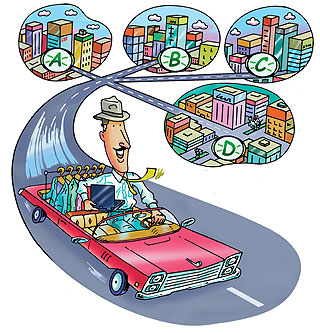
\includegraphics[width=0.9\textwidth]{billeder/forside.jpg}

\vspace{2cm} 
\textsc{\Large P1 Projekt \\
Gruppe A401 \\
Software\\
Aalborg Universitet\\
Den. 18. December 2014\\}
\end{flushright}

\cleardoublepage												% Indsaetter tom side, saa naeste kapitel starter paa hoejre side (hvis noedvendigt)
% Dette er LaTeX-versionen af titelbladet for TNB studenterrapporter
% Filen kræver:
% Universitetets logo:  AAU-logo-stud-UK eller AAU-logo-stud-DK
% Synopsis: En fil ved navn synopsis.tex

% Udarbejdet af: Jesper Nørgaard (jesper@noergaard.eu) 10. april 2012

\phantomsection
\pdfbookmark[0]{Titelblad}{titelblad}
\thispagestyle{empty}

\begin{minipage}[t]{0.48\textwidth}
\vspace*{-25pt}			%\vspace*{-9pt}

\includegraphics[height=4cm]{billeder/AAU-logo-stud-DK-RGB}
\end{minipage}
\hfill
\begin{minipage}[t]{0.48\textwidth}
{\small 
\textbf{Første Studieår v/ Det Teknisk-}\\
\textbf{Naturvidenskabelige Fakultet}  \\
Software \\
Strandvejen 12-14 \\
9000 Aalborg \\}
\end{minipage}

\vspace*{1cm}

\begin{minipage}[t]{0.48\textwidth}
\textbf{Titel:} \\[5pt]\bigskip\hspace{2ex}
Ruteplanlægning

\textbf{Projekt:} \\[5pt]\bigskip\hspace{2ex}
P1-projekt

\textbf{Projektperiode:} \\[5pt]\bigskip\hspace{2ex}
Oktober 2014 - December 2014

\textbf{Projektgruppe:} \\[5pt]\bigskip\hspace{2ex}
A401	

\textbf{Deltagere:} \\[5pt]\hspace*{2ex}
Christian Dannesboe \\\hspace*{2ex}
Frederik Børsting Lund \\\hspace*{2ex}
Karrar Al-Sami \\\hspace*{2ex}
Mark Kloch Haurum \\\hspace*{2ex}
Mikael Aarsnes \\\hspace*{2ex}
Rabee Mohamad Kaddoura \\\bigskip\hspace{2ex}
Søren Lyng

\textbf{Vejledere:} \\[5pt]\hspace*{2ex}
Mona-Lisa Dahms \\\bigskip\hspace{2ex}
Jane Billestrup

\vspace*{1cm}

\textbf{Oplagstal: 10} \\
\textbf{Sidetal: 80} \\
\textbf{Appendiks: 3} \\ 
\textbf{Afsluttet 18-12-2012}

\end{minipage}
\hfill
\begin{minipage}[t]{0.483\textwidth}
Synopsis: \\[5pt]
\fbox{\parbox{7cm}{\bigskipProjektet er udafbejdet ud fra projektoplægget "Bedre rutevejledning i Google Maps". Frem for en rute mellem ét punkt til ét andet punkt, ønkes en flerpunktsrute. Som case har gruppen overvejet forskellige grupper, hvor valget faldt på at fokusere på turister. Formålet med projektet er at lave en interessant flerpunktsrute, dog vil gruppen ikke diktere hvad den interessante rute er, derfor kan brugeren selv tilføje attraktioner, som vil udgøre personens interessante rute. Der er blevet undersøgt forskellige algoritmer, til at finde en relativ kort rute mellem attraktionerne, så ruten både vil være brugerens interessante rute, samt den forholdsvis korteste rute.
\bigskip}}
\end{minipage}

\vfill

{\footnotesize\itshape Rapportens indhold er frit tilgængeligt, men offentliggørelse (med kildeangivelse) må kun ske efter aftale med forfatterne.}

% Rapportens indhold er frit tilgængeligt, men offentliggørelse (med kildeangivelse) må kun ske efter aftale med forfatterne.
% The content of the report is freely available, but publication (with source reference) may only take place in agreement with the authors.

%\cleardoublepage
\phantom{Luft}

\phantom{Luft}

\begin{table}[H]
	\centering
		\begin{tabular}{c c c}
			\underline{\phantom{mmmmmmmmmmmmmm}} & \underline{\phantom{mmmmmmmmmmmmmm}} & \underline{\phantom{mmmmmmmmmmmmmm}} \\
			Christian Dannesboe			& Frederik Børsting Lund 		& Karrar Al-Sami 			\\
			&&\\
			&&\\
			\underline{\phantom{mmmmmmmmmmmmmm}} & \underline{\phantom{mmmmmmmmmmmmmm}} & \underline{\phantom{mmmmmmmmmmmmmm}} \\
			Mark Kloch Haurum			& Mikael Sandegaard Aarsnes 		& Rabee Mohamad Kaddoura 				\\
			&&\\
			&&\\
		 							& \underline{\phantom{mmmmmmmmmmmmmm}} 	&			\\														
									& Søren Lyng 							& 												
		\end{tabular}
\end{table}
\newpage
\chapter*{Forord}

Forord yes yes

\textbf{Læsevejledning}

Sådan læses rapporten

\phantom{Luft}

\phantom{Luft}

\begin{table}[H]
	\centering
		\begin{tabular}{c c c}
			\underline{\phantom{mmmmmmmmmmmmmm}} & \underline{\phantom{mmmmmmmmmmmmmm}} & \underline{\phantom{mmmmmmmmmmmmmm}} \\
			Christian Dannesboe			& Frederik Børsting Lund 		& Karrar Al-Sami 			\\
			&&\\
			&&\\
			\underline{\phantom{mmmmmmmmmmmmmm}} & \underline{\phantom{mmmmmmmmmmmmmm}} & \underline{\phantom{mmmmmmmmmmmmmm}} \\
			Mark Kloch Haurum			& Mikael Sandegaard Aarsnes 		& Rabee Mohamad Kaddoura 				\\
			&&\\
			&&\\
		 							& \underline{\phantom{mmmmmmmmmmmmmm}} 	&			\\														
									& Søren Lyng 							& 												
		\end{tabular}
\end{table}
\cleardoublepage

%%%% Indholdsfortegnelse (TOC) %%%%

\phantomsection													% Kunstigt afsnit, som hyperlinks kan 'holde fast i'
\pdfbookmark[0]{Indholdsfortegnelse}{indhold}					% Tildeler en klikbar bookmark til den endelige PDF
\tableofcontents*												% Indholdsfortegnelsen (kaldet ToC) 

%\addtocontents{toc}{\protect\newpage}							% Fremtvinger sideskift i ToC hvis noedvendig (der hvor koden placeres)


\mainmatter														% Hovedindhold - nummereres fra side 1

%%%% Rapportindhold %%%% 										% Rapportindholdet boer IKKE indeholde broedtekst - KUN includede filer!

%% Indledende %%												% Opdel evt. i passende afsnit for overblikkets skyld

\chapter{Indledning}

Hvert år besøger flere millioner turister Danmark, hvilket er godt for den danske økonomi. Når turisterne bruger penge på en dansk vare, service eller oplevelse, bliver det sådan set eksporteret til udlandet – og derfor bliver dette betragtet som en eksportvare. I alt står denne eksport type for 3,6\% af den danske eksport. Turisterne har et forbrug på 87,2 mia. kr., hvoraf de udenlandske turister bruger 35,7 mia. kr. altså godt 41\%, mens de danske turister står for de resterende 59\%. Udover at turismen hjælper det danske samfund økonomisk, skaber turismen ifølge VisitDanmark knap 122.500 fuldtidsjobs. \citep{faktaogtalVD}  \newline
Det ses gerne at turisterne kommer tilbage til Danmark igen. Dette sker naturligvis ved, at turisterne nyder deres ophold og får den bedst mulige ferie. Som turist i en storby kan det forekomme svært at finde rundt, og samtidigt virke let at fare vildt. Hvis en turist i København gerne vil se Rundetårn, kan turisten kigge efter det store monument, og gå i den retning hvor attraktionen nu er. Dog kan det ske at turisten undervejs mister tårnet af syne, og pludseligt ved turisten ikke i hvilken retning personen nu skal gå. Turisten kan vælge at bruge sin smartphone, hvis turisten da er i besiddelse af en, og kan eksempelvis gå på internetsiden GoogleMaps. Dette har de danske turister mulighed for, men for en udenlandsk turist vil dataen de bruger på ferie, fra deres smartphone koste mere, end det ville hjemme i deres hjemland\citep{VF}.  Her kan turisten så finde en rutevejledning fra punkt A til B, dog vil der kunne opleves problematikker, hvis en flerpunktsrute ønskes. I dette projekt har gruppen valgt at afgrænse sig til at undersøge en enkelt dansk by, i dette tilfælde valgte gruppen Aalborg, da dette var mest oplagt.

For turisten vil planlægning på forhånd være en god ting, hvis turisterne vil nå så mange attraktioner som muligt på en ferie, da tiden kan være begrænset \citep{YouthCentral}. Hvis feriedestinationen er i udlandet, ville en offline løsning til ruteplanlægning være optimal, da brugen af mobildata i udlandet kan koste mange penge \citep {TDC}.\newline
Samtidigt kan der spørges, hvad der gør en rute god: Er det hvor hurtigt turisten kommer fra den ene valgte attraktion til den anden? Kan der findes en mere interessant rute, eventuelt med attraktioner der ikke er oplyst i rejsebureauets brochurer, måske en smutvej forbi havnen eller muligheden for en flerpunktsrute mellem attraktionerne? Der kan være mange parametre der spiller ind, når den foretrukne rute skal vælges.

I dette projekt har gruppen valgt at undersøge: \newline \textit{I hvilket omfang kan ruteplanlægning hjælpe turister med, at finde den hurtigste eller mest interessante rute mellem attraktioner i Aalborg?} \newline 
Herunder kan der undersøges hvad en interessant rute ville være, hvilken form for rute turisterne foretrækker og i hvilke situationer har turister brug for ruteplanlægning og hvorfor? Derudover vil gruppen undersøge hvilke typer af turister der er relevante i forhold til dette projekt og hvad deres behov kunne være. \newline 


\section{Begreber}
Ved en ’interessant rute’ vil der i denne rapport refereres til en rute, der indkluderer unikke kulturelle og nationale oplevelser, hvor det interessante aspekt er individuelt for hver turist. Steder der ville kunne gøre ruten mere interessant vil bl.a. være havnefronten, gågaden eller andre attraktioner turisten ikke selv havde tænkt på, som turisten ville kunne passere på sin vej fra A til B.\newline

En ’attraktion’ vil i denne rapport forstås som både traditionelle, og utraditionelle attraktioner. Traditionelle attraktioner i Aalborg er Aalborg Zoo, kunstmuseet og lignende. De utraditionelle indkluderer steder som Storcenteret, Ikea og Havnefronten.\newline

’Turist’ vil i denne rapport være til dels defineret ud fra UNWTOs (UN World Tourism Organistation) beskrivelse, som beskriver to slags turister. En-dagsturister, som maksimalt overnatter én nat på stedet, og en generel turist, som overnatter mere end en nat\citep{Turismen}. Udover disse to typer findes undergruppen ’erhvervsturister’. Dette er turister, der kommer til stedet med et arbejdsformål. \newline
En turist er en person, der har et bestemt formål med rejsen, til forskel fra besøgende og rejsende. Formålet kan fx være, at opleve den danske kultur. \newline

En ’storby’ i Danmark, er i denne rapport en by, omgivet af områder med lavere bebyggelse. Hvor Aalborg fx har Nørresundby og Vejgaard.

Med dette afsnit har gruppen dannet grundlag for analysen, hvori de beskrevne begreber vil blive brugt. I de kommende afsnit vil den initierende problemstilling og dets spørgsmål blive analyseret.
% Analyse % 

\chapter{Problemanalyse}
\section{Interessentanalyse}

Gruppen vil i dette afsnit kigge på diverse personer/grupper, der kan fungere som interessenter i projektet. Herefter vil gruppen prioritere disse interessenter, alt efter hvor relevante de er i forhold til projektet.

\subsection{Storbyturister}
Turisterne har er en interessent i projektet, da det er dem projektet retter sig imod. Det er turisterne der skal anvende ruteplanlægningen, til at forbedre deres ferie og derfor vil de være interesseret i at det fungere så godt som muligt. 
Storbyturister er en væsentlig interessent i projektet, da en turist i en storby ofte vil se en masse ting. Hvis turisterne ikke planlægger hvad det er, de vil se, kan turisterne meget nemt glemme at få besøgt nogle af de seværdigheder, de ville se. Det kan skyldes, at turisterne vælger at gå en meget lang rute, og derved finder andre ting som de vælger at bruge deres tid på, eller at de simpelthen bare ikke kan finde vej til den attraktion de nu ønsker at se. Et ruteplanlægningsværktøj vil derfor være interessant for storbyturister, da det kan være med til at planlægge den helt rigtige ferie, hvor turisterne kommer til at besøge alle de attraktioner, de ønsker at besøge.

\subsection{Statsejede/privatejede attraktioner}
Statsejede attraktioner er en interessent i projektet, da staten ønsker, at der skal flere penge ind i landet. Hvis der er turister i et land, vil staten være interesseret i at få turisterne til at se og prøve så mange attraktioner, der er i landet som muligt. På den måde vil der være flere penge til landet. 
De privatejede attraktioner vil ligeledes være en interessent i projektet, da private ejere ønsker at tjene så meget som muligt. 
Her vil et ruteplanlægningsværktøj kunne hjælpe turister med at se nogle af de attraktioner der er i landet, hvis der fx er en top 5 over de attraktionerne der er i landet, eller i den by ferien foregår.

\subsection{Forretninger} 
Diverse forretninger er også en interessent i projektet, da kendte brands som fx Adidas, H\&M, McDonald’s og lignende gerne vil tiltrække flere kunder. Ved at implementere disse adresser i et ruteplanlægningsværktøj, kan det tiltrække nysgerrige turister, og derved øge forretningernes omsætning. 
Dette kan dog komme til at gå udover de mindre forretninger i byerne, da der er en chance for, at de vil blive besøgt mindre, eftersom mange turister ikke nødvendigvis kender de mindre forretninger. 

\subsection{Turistkontoret}
Turistkontoret er også en interessent i projektet, da deres job er at servicere turister og hjælpe dem med at finde vej til diverse attraktioner. Et ruteplanlægningsværktøj kan potentielt udgøre en risiko for at der bliver mindre at lave i et turistkontor og derfor medføre nogle fyrringer. På den anden side kan det også hjælpe turister med at få hjælp, når nu turistkontoret har lukket, eller hvis der er for lange køer. 

\subsection{Guide-bureauer/pakkerejser}
De forskellige guide-bureauer der sælger pakkerejser med guide og lignende, er også en interessent i projektet. Disse bureauer vil være imod et ruteplanlægningsværktøj, da det kan fratage dem nogle potentielle kunder, og derved sænke guide-bureauernes indkomst.   

\section{Prioriteringen}
--- billede af matrixen indsættes ---
For at prioritere interessenterne i projekter, har gruppen valgt gøre brug af indflydelse/medvirken-matrixen. I matrixen er der fire underpunkter, kaldet gidsler, ressourcepersoner, ekstern og grå eminence.
Gidsler er interessenter i projektet, med en vigtig aktiv medvirken og lille indflydelse. Ressourcepersoner er interessenter i projektet, med en vigtig aktiv medvirken og stor indflydelse. Eksterne er interessenter i projektet, med en mindre vigtig aktiv medvirken og lille indflydelse. Grå eminence er interessenter i projektet, med en mindre vigtig aktiv medvirken, og stor indflydelse.

\subsection{Gidsler}
Gidslerne i projektet, er de stats-/privatejede attraktioner, de større butikker og storbyturisterne.
Disse interessenter er gidsler, da det uden deres interesse, vil være meget svært, at lave et ruteplanlægningsværktøj, der opfylder det turisterne har brug for. Grunden til at deres indflydelse på projektet ikke er stor, skyldes at adresserne ligger på nettet, så det er forholdsvist nemt at finde adresserne til attraktioner, butikker etc. uden deres hjælp. Grunden til at turisterne er gidsler, skyldes, at de ikke har meget indflydelse i projektet, de skal blot anvende ruteplanlægningsværktøjet.

\subsection{Ressourcepersoner}
Ressourcepersonerne i projektet, er turistkontoret.
Turistkontoret i dette projekt er ressourceperson, da de har rigtig mange informationer om turister, og hvad turisterne gerne vil se. Derudover kan de have idéer til hvad der skal indgå i gruppens program, for at det vil være mest optimalt for turisterne.   

\subsection{Ekstern}
De eksterne i projektet, er de små butikker og guide-bureauer.
Disse interessenter er på en måde ”ofrene” ved projektet. De har ikke særlig meget at skulle have sagt, og de har stort set ingen indflydelse på projektet, men projektet har en indflydelse på dem, og deres indkomst. 

\subsection{Grå eminence}
Gruppen har i dette projekt, ikke nogle interessenter der passer under denne kategori.


\section{Konklusion på interessentanalyse}

Ud fra interessenterne fra interessentanalysen, har gruppen vurderet, at der er to væsentlige store interessenter, i forhold til de andre. Disse to interessenter er turisterne og turistkontoret. 
Grunden til, at det er disse to, skyldes, at hvis gruppen senere hen skal udvikle et program, så mener gruppen, at det program skal rettes hen imod den ene eller den anden. Altså lave et ruteplanlægningsværktøj der har turisterne som fokus, hvor så det ville komme med forslag og idéer til hvad turisterne kan se i byen og lignende. Hvis det så derimod er turistkontoret, der er i fokus, kunne et program måske programmeres i forhold til turistkontorets ønsker, således, at turisterne vil komme tilbage til byen. 
Gruppen har besluttet, at fokusset i projektet, vil være turisterne frem for turistkontoret, da gruppen mener, at det er vigtigst, at turisterne får det bedste ud af deres ferie som muligt. 




\section{Spørgeskema}
I dette afsnit vil man kunne se udformningen af spørgeskemaet og de resultater som der vil kan uddrages fra spørgeskemaet. I interessesentanalysen blev turister placeret som en delvis resourceperson, og ud fra dette har gruppen valgt at lave et spørgeskema, som skal hjælpe med at besvare den initierende problemstilling. Dette blev gjort med den hensigt at få så mange synspunkter på de opstillede problemstillinger, så det ville være muligt at generalisere ud fra besvarelserne. Spørgeskemaet bliver udarbejdet vha. den kvantitative metode, i form af et internetinterview. Se i apendix X om mere information om den brugte teori og rådata.

\subsection{Udformning}
Først udformede vi en række problemstillinger vi ville have svar på i vores undersøgelse: 
\begin{itemize}
\item Hvilke slags attraktioner tager turister til storbyerne for at se?
\item Hvordan planlægger turister deres ferie?
\item Hvordan finder turister rundt?
\item Har turister problemer med at finde rundt?
\item Fortrækker turister den hurtigste eller den mest interessante rute?
\item Er den løsning vi har i tankerne noget respondenterne ville bruge?
\end{itemize}
Da gruppen havde valgt et internetinterview i form af en online undersøgelse, valgte gruppen at dele spørgsmålene på Facebook. Dette vil dog give nogle begrænsninger: Spørgeskemaet kan kun ses af personer som gruppen er venner med på Facebook, hvilket mest vil være unge mennesker. Derudover er spørgeskemaet lavet på dansk, for at gøre spørgsmålene så let forståelige som muligt for gruppens venner på Facebook. Da mange af de personer gruppen kender på Facebook sikkert ikke har været turister i Aalborg, blev spørgsmålene rettet mod alle storbyer.
\subsection{Resultatbehandling}
Spørgeskemaet var lagt op på Facebook i tre dage, hvorefter resultaterne blev behandlet. I alt var der kommet 60 besvarelser, hvilket giver gruppen en relativ lille respondentgruppe at arbejde med, dog giver resultaterne nogle klare tendenser, som gruppen har arbejdet ud fra. Herunder kan der ses forklaring på formålet med spørgsmålet, og hvad besvarelserne fortæller os.

\textbf{Hvad er vigtigt for dig på din storbyferie?}\newline
Formålet med dette spørgsmål er at finde ud af hvad turister gerne vil se eller opleve i en storby, for at kunne se hvad der eventuelt kunne implementeres i projektets løsning.\newline
Ud fra besvarelserne afgivet af respondent gruppen (som kan ses i apendix A2), kan der ses hvad respondenterne vægter højest på deres storbyferie: Se byens seværdigheder, opleve kulturen, maden og shopping. Derudover var der en del der havde kommentereret, at de kom til storbyen for at se sportsbegivenheder. Dette var dog ikke en valgmulighed på spørgeskemaet, så det kan ikke uddrages til projektet, da mange respondenter måske ikke havde tænkt over denne mulighed.\newline

\textbf{Hvilke hjælpemidler bruger du til at planlægge din storbysferie?}\newline
Formålet med dette spørgsmål er, at finde eksisterende planlægningsværktøjer, hvor der kunne kigges på fordele og ulemper til dette projekt.\newline 
I besvarelserne kan der ses en liste af eksisterende planlægningsværktøjer, hvor de både er elektroniske og i form af brochurer og lignende.\newline
 
\textbf{Hvilke redskaber bruger du til at finde rundt når du er på storbyferie?}\newline
Formålet med dette spørgsmål er at finde ud af om turister brugte redskaber til at finde rundt.\newline 
Ud fra besvarelserne på dette spørgsmål kan der ses, hvilke redskaber respondentgruppen bruger, til at finde rundt på ferier. Her har respondentgruppen mulighed for at svarer på mere end én ting. Der kan ses at 81,67\% bruger diverse kort og brochurer, og 55\% bruger elektroniske redskaber til at finde rundt. \newline

\textbf{Har du nogensinde haft problemer med at finde vej på din storbyferie?}\newline
Formålet med dette spørgsmål er at få afklaret om et af de problemer vi opbygger vores projekt omkring, faktisk er et problem.\newline
Ud fra besvarelserne kan der ses, at hele 68,33\% altså hele 2/3, har haft problemer med at finde rundt på deres storbyferie.\newline

\textbf{Når du skal fra en aktivitet til en anden på din storbyferie, vil du helst tage den hurtigste rute eller en langsommere men mere interessant rute?}\newline 
Formålet med dette spørgsmål er, at finde ud af hvad turisterne helst ville have, en hurtig rute fra A til B, eller en interessantrute, som er langsommere, hvor man får set andre ting på vejen  til sin destination.\newline
Der ses tydeligt at vores respondenter fortrækker den interessante rute over den hurtigste rute, med henholdsvis 80\% for den interessante og 20\% for den hurtigste. Folk er mere interesseret i at få flere oplevelser, end at komme hurtigt frem til næste punkt på dagsordenen.\newline

\textbf{Et program/applikation, som hjælper mig med at finde den hurtigste og/eller mest interessante vej igennem byen, via mine valgte ”must see” destinationer, ville være noget jeg kunne bruge?}\newline
Formålet med dette spørgsmål er at finde ud af om projektet egentlig har nogen interesse hos brugeren.\newline  
I dette spørgsmål svarede 90\% at den ideelle løsning ville enten kunne bruges eller ønskes. \newline

\chapter{Interview}
\section{Teori}
Der er mange former for interviews og disse kan udføres på forskellige måder, men typisk når der snakkes om interviews, bliver de delt ind i tre forskellige former, enkeltinterview, spørgeskemaer og telefoniske interviews.
Dette afsnit er udarbejdet ud fra PDF'en om dataindsamling, der kan ses i litteraturlisten, under \citep{metodeogprojektskrivning}.\newline

\textbf{Enkeltinterview}\newline
Det enkelte interview forgår på følgende måde: Både intervieweren og respondenten mødes ansigt til ansigt. Fordelene herpå er tydelige, at give respondenten mulig for at besvare private og intime spørgsmål, som en almen respondent ikke er tryg ved at tale om foran andre. Dette mindsker også chancen for at spørgsmålene bliver misforstået, samtidig med at svarene kan diskuteres på et højere plan, end ved et interview over telefonen eller ved et spørgeskema, da snakker med mere end bare ord, nemlig kropssprog. Hvis intervieweren har en god situationsfornemmelse kan et vellykket interview, forventes. 
En udvidelse af enkeltinterviewet kan der snakke om gruppeinterview. Metoden bruges hvis der er pres på tid og ressourcer. Metoden er den samme udover den forskel at der er flere respondenter. Der opfordres ikke til dialog mellem respondenterne. Et modsvar til denne metode er fokusgrupper. Denne metode opfordre netop til dialog mellem respondenterne, men emnet her er temmelig afgrænset. Denne metode bliver brugt til at sammenligne skabelsen af holdninger i sociale miljøer og hvilke argumenter der bliver taget i brug. \newline

\textbf{Telefoninterview}\newline
Det telefoniske interview er lidt en sammenblanding af de to ovennævnte interview former. Telefoninterviewet foregår ved at en eller flere interviewere sidder bag røret og stiller en række spørgsmål, som på forhånd er fastlagte. Den væsentlige forskel på telefoninterviewet som er et kvalitativt interview og spørgeskemaet som er et kvantitativ interview, er at interviewerne kan uddybe deres spørgsmål på et højere plan, end et spørgeskema vil kunne. Måden hvorpå denne form for interview foregår er ved at scanne spørgeguiden ind i et program, hvorefter dette vil blive sendt til respondenten og unødvendige spørgsmål undgås. Her har respondenten så mulighed for at skrive sine egne svar ind, hvilket mindsker fejl ved fx transskription. Til sidst har intervieweren mulighed for at gå i detaljer med hvert spørgsmål sammen med respondenten.\newline

\textbf{Spørgeteknikker og metoder til interview}\newline
Når der snakkes om videnskabelige spørgeteknikker er det vigtigt at kende forskellene på dette og dagligdagssproget, som normalt bliver snakket. Der er de standardiserede spørgeteknikker, hvilket er hvor spørgsmålene og rækkefølgen på disse, omhyggeligt er blevet arbejdet med, og deres rækkefølge, er valgt på forhånd for interviewet. Denne metode er nyttig at tage i brug, hvis en interviewer kender problemstillingen. Her får intervieweren svar på sine spørgsmål med så lidt spildt information som muligt. Dette udføres typisk med spørgeskemaer. Nogle forskere mener, at et standardiseret interview også har det element, at forholdene og endda tiden for interviewet er ens for alle respondenter. Alle andre former for interview er indenfor kategorien ikke-standardiseret interview.
Derudover er der de strukturerede interviews. Dette forgår lidt på samme måde, som de standardiserede interviews. Den væsentligste forskel herpå, er at spørgsmålene ikke er fastlagte, så det kun er spørgeguiden, der er fastsat. Dette skaber større mulighed for en kvalitativ interviewform, hvor intervieweren kan følge op på emner der kommer, som intervieweren ikke havde regnet med. Som et modsvar på denne form for interview, findes det ikke-strukturerede interview. Denne metode har hverken fastlagte spørgsmål, eller en fastlagt spørgeguide/rækkefølge på spørgsmål. Ved brug af denne metode kan intervieweren frit følge et givent emne ud fra respondentens svar, derfor kaldenavnet  ”det fleksible interview”.\newline
 
\textbf{Lukkede og åbne spørgsmål}\newline
Lukkede spørgsmål bruges typisk ved kvantitative spørgeteknikker såsom et spørgeskema. Altså teknikker som gør at responsen let kan sammenlignes og analyseres. Denne metode af spørgsmål falder altså ind under kategorien standardiseret spørgsmål, da respondenten hverken kan ændre på rækkefølgen af spørgsmålene eller gå ind og uddybe sine svar. 
Til hvert et træk, er der et modtræk. De åbne spørgsmål, som bliver benyttet i de kvalitative aspekter indenfor spørgeskemaer, altså den mulighed at respondenterne kan uddybe nogle svar, hvis intervieweren føler det er nødvenligt og stille sådan en plads til rådighed i spørgeskemaet.\newline

\textbf{Psykologiske teknikker}\newline
Interviewerens situationsfornemmelse er kritisk ved at ansigt-til-ansigt interview, altså at intervieweren kan fornemme atmosfæren, hvilke ting intervieweren kan spørge om og hvilke intervieweren ikke kan. At intervieweren kan læse respondentens kropssprog, når spørgsmålene bliver stillet, kan bruges til fordel for interviewet. Hvis dette bliver ignoreret, kan det ende med et mislykket interview.\newline

\textbf{Passive teknikker}\newline
Denne teknik går ud på at stille et spørgsmål, lade respondenten svare, hvorefter intervieweren kommer ind med nogle spørgende kommentar. Ved brug af denne teknik, mindskes interviewerens bestemmelse i retningen af interviewet, og respondenten kan komme med mere information, om et givent emne, og endda indbringe egne meninger og holdninger, hvis dette er vigtigt ift. emnet.\newline

\textbf{Tive teknik}\newline
Hvis respondenten ikke er specielt snakkesalig kan intervieweren give ham/hende følelsen af at den viden de har, er interessant og vigtig, ved fx at spørge, ”Jeg synes dine iagttagelser er interessante” o. lign.\newline

\textbf{Aktiv spørgeteknik}\newline
Hvis intervieweren kommer ud for, at respondenten er meget sky og tilbageholden med information, kan intervieweren manipulere ham/hende til at tro at den information de kommer ud med, er en lille del af en manglende kæde. Fx kan intervieweren nævne en given situation, hvorefter intervieweren spørger ind til det manglende led, altså den information intervieweren mangler. På denne måde ligner respondentens svar ”bare” et lille manglede led i noget intervieweren allerede ved.\newline

\textbf{Interviewet}\newline
Inden vores interview stillede vi nogle spørgsmål op, som der gerne skulle besvares til vores interview med Lars. Disse spørgsmål var skrevet med henvisning af vores underspørgsmål i problemindledning, så vi gerne skulle kunne få noget henblik og svar til vores spørgsmål. Ud over det, ville vi gerne have noget, information omkring turismen i Aalborg, for at se om emnet kunne have relevans for turister i Aalborg. 
Interviewet var sat op til at være et enkeltinterview, og med passive spørgsmål til. Med det ville vi gerne stille vores spørgsmål, hører hvad Lars havde at svare til det, og herefter komme med uddybende spørgsmål, eller få en samtale i gang omkring emnet. Denne teknik blev valgt, fordi at der på den måde måske kunne komme andre ting ind, som gruppen måske ikke havde tænkt på. Så ved denne teknik lader vi Lars tale frit, og komme med alle de ting, han tænker der kunne have relevans for emnet. Vis der i stedet havde brugt lukkede spørgsmål, ville vi kun få dækket det som gruppen havde tænkt på, og måske mistet noget viden Lars havde, der kunne have været relevant for emnet. 
Selve interviewet, forgik meget mere frit, end det var planen. Der blev stillet nogle få af de spørgsmål, som der var lavet på forhånd, men fik ikke stillet dem alle sammen. Lars var rigtig god til at have en samtale i gang, og det slog lidt spørgsmålene til siden, og blev mere en samtale omkring turismen i Aalborg, og Visit Aalborgs situation i turismen. Så interviewet gav et større indblik i turismen i Aalborg, men ikke så mange ideer til løsningsforslag.
\section{Eksisterende løsninger}
I spørgeskemaet blev der opremset en række af hjælpemidler som respondenterne bruger på deres storbyferie, hvilket til projektet vil være eksisterende løsninger. I det kommende afsnit vil der blive analyseret på TripAdvisors app, hvilken var en af de hjælpemidler som respondent gruppen havde nævnt. Der udover har gruppen fundet Fidnthebestrute.com, som vha. Google Maps kan lave en flerpunktsrute.  

\subsection{TripAdvisor Offline City Guides}
TripAdvisor har en offline app, der kan hjælpe med at guide turister rundt, i den by de er rejst til. Den har mange forskellige funktioner, som fx et kort indlagt i appen. Dette kort kan være effektivt, hvis brugeren har forberedt sig hjemmefra. Dette skyldes, at turisten kan downloade et kort over den by, brugeren skal besøge, og derved vil den fungere offline. Grunden til at det er effektivt for turister, skyldes at mobildata kan være dyrt i udlandet\citep {TDC}. \newline
Udover et kort, har app'en også nogle informationer omkring de mange forskellige byer. Disse informationer har turisten ligeledes mulighed for at downloade, så de også er tilgængelige offline. Ved hjælp af disse informationer, kan turisten fremskaffe sig hjælp, hvis turisten fx er interesseret i at finde en restaurant, et hotel, se en bestemt attraktion eller lignende. Ønsker brugeren fx at besøge en attraktion, kan der ved hjælp af en knap, klikkes frem til en lokation, som turisten enten selv kan finde vej til, eller benytte en anden knap i app'en og få indlagt ruten i det downloadede kort.\newline
Hver af disse kategorier indeholder en ”Best in Town”-funktion, som er en liste over de mest populære attraktioner, ifølge TripAdvisors brugere, da der er et point-system, som giver brugere af app'en mulighed for at vurdere og skrive kommentar til de enkelte attraktioner, på en skala fra 1-5. \newline
TripAdvisors app har mange gode funktioner. En af de gode funktioner, er det offline kort, der giver mulighed for at undgå brugen af mobildata på en udlandsrejse, og gør det muligt hele tiden at have et kort ved hånden. Herudover kan der fås et indblik i, hvilke ting der er at se og opleve i den valgte by, med kommentarer og ratings fra andre brugere, der har besøgt disse steder.
Appen har også nogle mangler, som fx at vælge flere seværdigheder på listen, og give en rute mellem disse seværdigheder, så det er muligt at få en flerpunktsrute. \newline
\subsection{FindTheBestRoute.com}
Google Maps er begrænset til kun at kunne vise vejen fra et punkt til et andet. Det har FindTheBestRoute.com taget kampen op imod, og har derfor lavet en hjemmeside på FindTheBestRoute.com, hvor den korteste rute mellem maksimalt 10 forskellige adresser kan beregnes. FindTheBestRoute.com, udnytter Google Maps JavaScript API v3, altså en grænseflade til Google Maps, der tillader andre programmer at benytte Google Maps, til fx at få vist et kort, eller beregne en rute \citep{ftbr}.\newline
Selvom der på maps.google.dk ikke er mulighed for at indtaste forskellige destinationer, og få anvist den korteste rute imellem punkterne, så har Google Maps allerede funktionaliteten indbygget til at foretage denne beregning, som en løsning på ”The Travelling Salesman Problem”.\newline
For findthebestroute.com, er det derfor simpelt at sende en anmodning til Google, der indeholder informationer om de forskellige destinationer der skal forbindes med en rute. Google foretager så beregningerne, og sender den bedste rute tilbage til findthebestrute.com, hvor de så kan vise ruten til deres brugere \citep{googleapi}. \newline
\subsection{Opsummering}
TripAdvisor har mange gode funktioner, så som offline kort, "Best in Town" og information om de enkelte attraktioner. TripAdvisor findes som en app, så den er tilgængelig på ferien. TripAdvisior har dog ikke mulighed for at lave en flerpunktsrute. \newline
FindTheBestRoute.com har intet af det som Tripadvisor har, den har dog muligheden for at lave en flerpunktsrute, med maksimalt 10 adresser. Problemet med FindTheBestRoute.com er at den kun er tilgængelig på internettet og derved er den mere besværlig på ferien.\newline
Disse synspunkter kan bruges til at udforme krav til projektets løsning. \newline

Næste afsnit vil omhandle problembeskrivelsen, som indeholder problemafgrænsningen og den endelige problemformulering. 


% Problem %
\chapter{Problembeskrivelse}

I dette afsnit vil den endelige problemformulering blive beskrevet.

\section{Problemafgrænsning}
Ud fra denne analyse, kan der konkluderes, at VisitAalborg og turisterne er ressourcepersoner, hvoraf turisterne har større indflydelse på programmet, da de er de endelige brugere. VisitAalborg kan bruges som guider til, hvad der kan være af indhold i programmet, men der skal stadig tages højde for, at det er i deres interesse, at få deres arbejdspartnere med ind i programmet, selvom det ikke i alle tilfælde er til turistens interesse.
Ved spørgeskemaet blev der uddraget, at turister allerede har løsninger fra punkt til punkt, hvor der i eksisterende løsninger blev påpeget, at der også findes løsninger for flerpunktsruter. TripAdvisor viste, at der også er programmer, som tager højde for brugerens interesse, men alt taget i betragtning, er der ikke en løsning der kombinerer alle disse funktioner, som der belyses i gruppens spørgeskema og interview, til at være i brugerens bedste interesse: En simpel løsning, der inddrager brugerens interesse, og foreslår yderligere punkter til en mere interessant rute. Dette kunne endda optimeres ved en offline-funktion, som TripAdvisor også gør brug af ved et offline kort.

\section{Problemformulering}
Hvordan udvikles der en softwareløsning, der hjælper turisten med at finde rundt i en storby, på en interessant rute mellem turistens egne valgte attraktioner?
\begin{itemize}
	\item Hvordan kan programmet finde en rute?
	\item Hvordan kan programmet gøre ruten interessant?
	\item Hvordan kan programmet hjælpe brugeren med at finde rundt?
\end{itemize}


% Problemlosning %

\chapter{Kravspecifikationer}
I dette afsnit vil gruppen vurdere, hvilke krav der skal indgå i en løsning. Heri vil der både blive opstillet krav til en optimal løsning og til en afgrænset løsning, som gruppen mener vil være realistisk, at kunne lave.

\section{Optimale løsningsforslag}
For at kunne udvilke en softwareløsning, der besvarer gruppens problemformulering, er det vigtigt at definere nogle krav til programmet. Til en optimal løsning, har gruppen vurderet, at der skal være følgende krav:
\begin{itemize}
	\item Programmet skal udvikles som en applikation til moderne smartphones, inklusiv iOS, Android og Windows Phone.
	\item Programmet skal hjælpe brugeren, til at lave en interresant rute gennem byen, vedkommende vil besøge.
	\item Programmet skal vise et overskueligt og scalerbart kort med ruten.
	\item Ruten skal udskrives i samme stil som Google Maps.
	\item Programmet skal kunne give rutevejledning undervejs på ruten. 
	\item Programmet skal kunne  downloade en offline version af den rute der er valgt, inklusiv kortet for det omkringliggende område.
\end{itemize}
Til disse krav har gruppen konstrueret nogle skitser og en beskrivelse af den optimale løsning, for at give et billede af hvordan det eventuelt kunne se ud. \newpage

Gruppen har valgt at lave den ideelle løsning på følgende måde:\newline
\newline
Brugeren bliver præsenteret for en liste over alle attraktioner i byen, sorteret efter afstand fra brugerens nuværende position, alfabetisk rækkefølge eller rating. \newline
Ratingen vil blive fundet ved at tage gennemsnittet af alle brugeres rating af den specifikke attraktion. Dette gøres for at give brugeren mulighed for at vælge de attraktioner vedkommende gerne vil se.
\newline
Programmet skal under udvælgelsen give brugeren mulighed for at læse om de enkelte attraktioner, så brugeren kan foretage informerede beslutninger om til- og fravælgelse af attraktioner.\newline
\newline
Når brugeren har valgt de attraktioner vedkommende vil besøge, udformes et kort med den korteste rute mellem disse attraktioner. På dette kort vil alle attraktioner som ligger indenfor en forudbestemt afstand til ruten, blive vist. Derefter kan brugeren tilføje nogle ekstra attraktioner, som vil blive tilføjet til den endelige rute.\newline
Dette gøres så brugeren kan udforme en mere interessant rute. Gruppen vil ikke diktere hvad den interessante rute er, men lade brugeren selv tilvælge, og derved få deres egen unikke interessante rute. \newline 


\begin{wrapfigure}{r}{0.3\textwidth}
	\vspace{-20pt}
	\begin{center}
		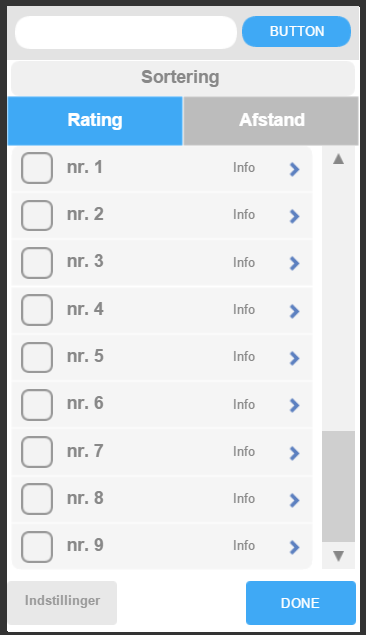
\includegraphics[scale=0.35]{start1} \newline
		\textit{Figur 4.1: Brugergrænseflade}\newline
	\end{center}
	\vspace{-20pt}
	\vspace{-20pt}
\end{wrapfigure}


Den optimale løsning vil som startside have en liste over alle attraktionerne. Disse skal kunne sorteres, til det findes to valg muligheder, forholdsvis rating og afstand, hvoraf rating viser en attraktionerne i rækkefølgen, baseret på hvad tidligere brugere har valgt at rate den. Funktionen afstand, vil vise hvor stor en afstand der er fra det punkt hvor brugeren står, til en attraktion. Attraktionerne vises da således, at den nærmeste attraktion er øverst. De attraktioner, som brugeren ønsker at se, skal brugeren blot trykke/klikke på og et flueben vil så komme frem i boksen til venstre. Efter alle de ønskede attraktioner er valgt, trykkes på done for at komme videre. Figur 4.1 viser en skitse af brugergrænsefladen. \newline
\newline
\newline
\newline

\begin{wrapfigure}{l}{0.3\textwidth}
	\vspace{-40pt}
	\begin{center}
		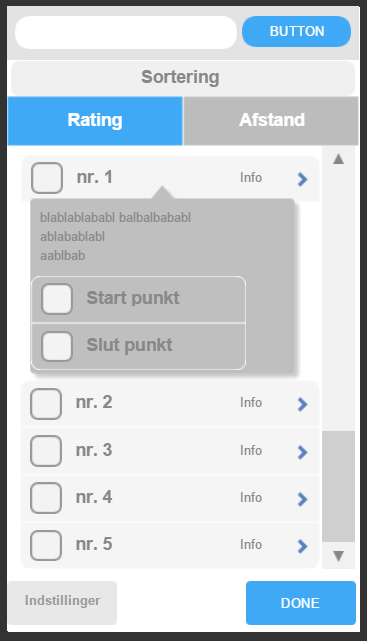
\includegraphics[scale=0.35]{start2} \newline
		\textit{Figur 4.2: \newline Eksempel på dropdown boks}\newline
	\end{center}
	\vspace{20pt}
\end{wrapfigure}

Hvis brugeren øsnker mere information om en bestemt attraktion, vil vedkommende have mulighed for at trykke på "info" eller den lille pil i højre side. Dette vil få en dropdown boks til at komme frem med information om attraktionen. Derudover vil der i denne boks, være mulighed for at vælge et start- eller slutpunkt. Disse punkter skal give brugeren mulighed for at vælge, hvor brugeren ønsker at starte/slutte sin rute. Figur 4.2 viser en skitse af denne dropdown boks.\newline
\newline
\newline
\newline
\newline

\begin{wrapfigure}{r}{0.3\textwidth}
	\vspace{-30pt}
	\begin{center}
		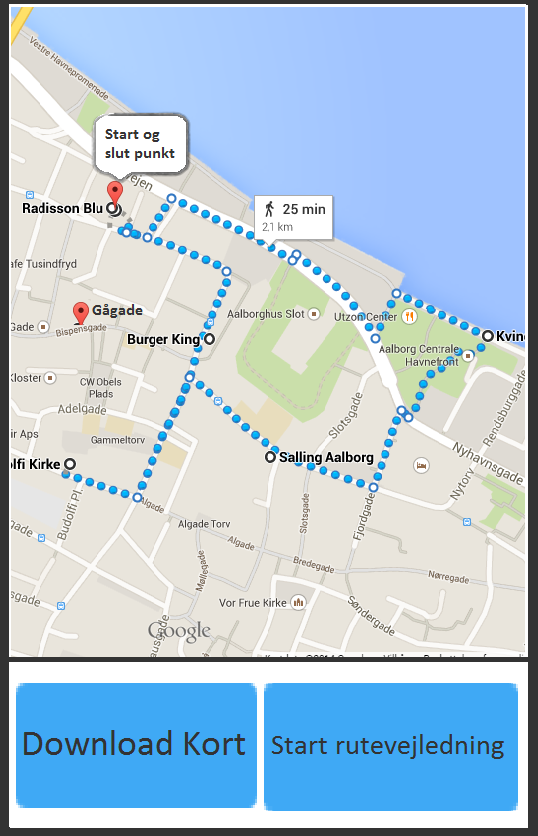
\includegraphics[scale=0.3]{rute1} \newline
		\textit{Figur 3.3: Rute - Ruten er\newline hentet fra Maps.Google.com}\newline
	\end{center}
	\vspace{0pt}
	\vspace{-100pt}
\end{wrapfigure}


Når der er valgt nogle ønskede destinationer/attraktioner, og trykket done på forige side, skal programmet fremvise et kort med en rute mellem de valgte punkter. Ruten skal vise hvor lang hele ruten er, og hvor lang tid det tager at gå ruten. På kortet skal der ydermere vises de attraktioner som ligger indenfor en hvis afstand til ruten. Disse vises som punkter med et navn tilknyttet.
Der skal desuden være to funktioner, når ruten bliver vist. Der skal være mulighed for at downloade kortet på mobilen, og derved gør det muligt at anvende programmet, uden brug af internet. Den anden funktion skal starte rutevejledningen, som fungere som en ganske almindelig GPS-rutevejledning. En skitse af dette kan ses på figur 4.3.\newline
\newline
\newline
\newline

\begin{wrapfigure}{l}{0.3\textwidth}
	\vspace{-60pt}
	\begin{center}
		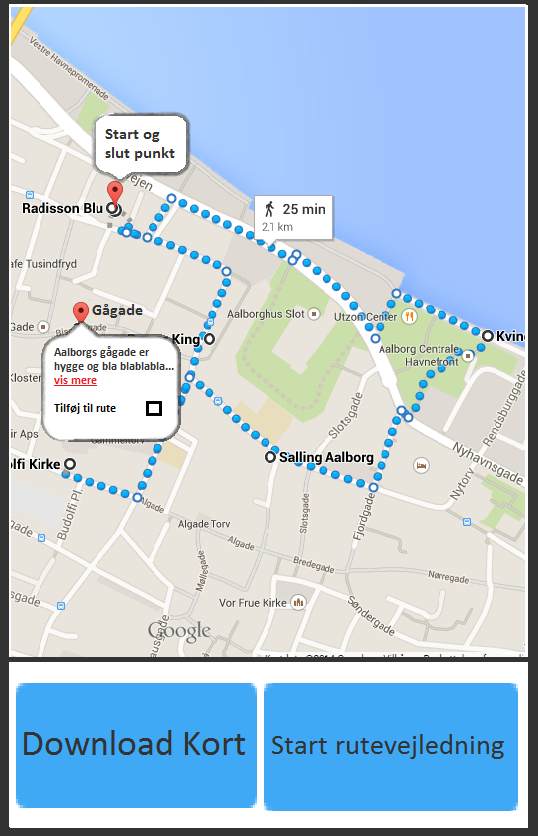
\includegraphics[scale=0.3]{rute2} \newline
		\textit{Figur 4.4: Udvidet rute - Ruten er hentet fra\newline Maps.Google.com}\newline
	\end{center}
	\vspace{-20pt}
	\vspace{-10pt}
\end{wrapfigure}

Når brugeren trykker på de attraktioner som er med på kortet, men ikke med i ruten, dette er, som beskrevet ovenfor, de attraktioner som ligger indenfor en hvis afstand til ruten, vil en boks komme frem med informationen om den givne attraktion. Der vil også være mulighed for her at tilføje denne attraktion til ruten. Figur 4.4 viser hvordan det eventuelt kunne laves. \newline
\newline
\newline
\newline
\newline
\newline
\newline
\newline
\newline
\newline
\newline


\section{Gruppens løsningsforslag}
Gruppen har gennem spørgeskema og interview fået stillet en række krav til løsningen, af respondentgruppen og VisitAalborg. 
Gennem spørgskemaet, blev det konkluderet, at det vigtigste for turister, er at de kan opleve byen på en interessant rute. 
Derudover har turistbureauet givet udtryk for, at løsningen gerne skal være så enkelt som muligt, altså færrest mulige funktioner, så brugeren ikke bliver forvirret, da de mener, at det er i turistens bedste interesse. \newline
Der er blevet stillet krav fra universitets side, om at programmet skal være et lille specifikt program i C, af høj kvalitet. Dette stemmer godt overens, med de krav der er blevet stillet fra turistbureauets side.   \newline
Ud fra dette, har gruppen opsat nogle krav for gruppens løsningsforslag, og de er som følgende:
\begin{itemize}
	\item Programmet skal kunne beregne en kort rute mellem en række punkter.
	\item Programmet skal beregne om der ligger en attraktion mindre end 100 meter fra ruten, og tilføje ekstra attraktionen til ruten, hvis brugeren ønsker det.
	\item Programmet skal som output give en liste over rutens destinationer, i den rækkefølge de skal besøges, i forhold til den korte rute.
\end{itemize}

Da dette er et P1 projekt, og gruppen er begrænset af både tid og erfaring, har gruppen valgt at begrænse softwareløsningen, på følgende punkter: 
\begin{itemize}
	\item Afstanden mellem attraktioner vil blive beregnet i fugleflugtslinje.
	\item Brugeren kan kun vælge destinationer ud fra en række forudbestemte punkter.
	\item Tekstbaseret brugergrænseflade.
\end{itemize}

På baggrund af kravene og afgrænsningen, har gruppen valgt at lave et program, som har nogle forudbestemte destinationer, der dækker over attraktioner i Aalborg, hvorefter brugeren vælger de attraktioner vedkommende ønsker at besøge. Programmet vil ud fra disse punkter, beregne en kort rute, og undersøge om der er andre attraktioner, som ligger tæt på ruten, og spørge brugeren, om det kunne være interessant at besøge disse steder. Hvis ja, vil disse punkter også blive inkluderet. På den måde får brugeren selv lov til at skabe sig den mest interessante rute. Resultatet bliver en liste over destinationerne, der står i rækkefølge, så turisten ved hvilken rækkefølge de skal besøge dem i, for at få den mest optimale rute.\newline

Det næste afsnit vil omhandle de teorier, som beskriver de formler, algoritmer og metoder, der er brugt i løsningen.

bn\chapter{Test}
For at sikre at programmet kører stabilt, og laver de korrekte udregninger, testes programmet for forskellige testcases. Der er forskellige metoder at teste dette på, hvoraf testen i denne rapport er blackbox testing. Denne testtype behandler en mængde testcases, som beskrevet i tabellen, hvor et bestemt input har et forventet output, og programmet testes derefter. Hvis det forventede output stemmer overens med det reelle output fra programmet, kan testen konkluderes succesfuld. 
En anden testtype kan være CU-test, som er et indlejret test-system, hvor testcases bliver oprettet som kode i programmet. Derefter vil testen blive kørt ved compile-time og resultater fra testcases bliver printet ud. Begrundelsen for brug af blackbox testing er, at der i dette program bliver printet gennem processen, og alle valg i programmet bliver foretaget af brugeren. Blackbox testing vil derfor give et godt billede, af om testen og input fra brugeren stemmer overens.

Casene er opbygget således:\newline
\begin{tabular}{|l|l| p{5cm}|}
	\hline
	Case 1 & Korrekt valgt af attraktioner & Korrekt tilføjelse af interessante punkter \\ \hline
	Case 2 & Korrekt valgt af attraktioner & For mange tilføjelser af interessante punkter \\ \hline
	Case 3 & Korrekt valgt af attraktioner & Forkert input-type ved tilføjelser af interessante punkter\\ \hline
	Case 4 & Korrekt valgt af attraktioner & Ingen tilføjelse af interessante punkter (input ”0”) \\ \hline
	Case 5 & Valg af flere attraktioner end muligt & Forventer ikke prompt for andet input\\ \hline
	Case 6 & Valg af samme attraktion flere gange &	Forventer ikke prompt for andet input\\ \hline
	Case 7 & Forkert input-type til valg af attraktioner & Forventer ikke prompt for andet input\\ \hline
	Case 8 & Intet valg af attraktion (første input ”0”) & Forventer ikke prompt for andet input\\ \hline
\end{tabular} 
\newline

\textbf{Case 1:} \newline
I denne første testcase, vil inputtet til valg af attraktioner være 1, 5 og 9. Ved brug af disse tal, vil et forventet output være Aalborghus\_Slot for 1, Springeren\_-\_Maritimt\_Oplevelsescenter for 5 og Nordkraft for 9. Herefter ville valget af attraktioner afsluttes, ved input 0.
Output ved første del af testcasen blev følgende: ”Tilfoejet attraktion: Aalborghus\_slot”, ”Tilfoejet attraktion: Springeren\_-\_Maritimt\_Oplevelsescenter” og ” Tilfoejet attraktion: Nordkraft”. Herved gav den første del et korrekt output. Ved afsluttelse af valg af attraktion, tilføjes disse attraktioner til ruten, og næste trin er tilføjelse af interessante, nærliggende attraktioner. Eftersom de valgte attraktioner alle ligger tæt på havnen i Aalborg, vil andre interessante attraktioner være Utzon Centeret, Havnefronten og Friis, da disse alle ligger tæt på en tiltænkt rute fra Nordkraft til Springeren, hvor Aalborghus Slot også besøges.\newline
Her foreslår programmet følgende: 1: Utzon\_Centeret, 2: Friis\_Aalborg\_Citycenter og 3: Havnefronten. Dette er et korrekt output efter de attraktioner der blev valgt. Disse er alle tre inden for en afstand af 100 meter fra enten den nuværende rute eller de valgte attraktioner. Efterfølgende skal brugeren selv vælge, om han vil tilføje disse attraktioner til ruten. I dette tilfælde bliver inputtet 1 og 2, for tilføjelse af Utzon\_Centeret og Friis\_Aalborg\_Citycenter. Outputtet blev ”Tilfoejet attraktion: Utzon\_Centeret” og ”Tilfoejet attraktion: Friis\_Aalborg\_Citycenter”. Dette stemmer overens med det forventede output, og tilføjelsen afsluttes med input 0. Herefter vil ruten blive dannet, og alle attraktioner valgt vil blive printet ud som ”Din rute”. Heraf vil der vises Aalborghus Slot, Springeren, Nordkraft, Utzon Centeret og Friis. Disse vil sorteres efter hvornår på ruten de besøges, hvor startpunktet vil blive printet dobbelt, som både start-attraktion og slut-attraktion. Siden startattraktionen er Aalborghus\_Slot, skal ruten blive Aalborghus\_Slot, Utzon\_Centeret, Friis\_Aalborg\_Citycenter, Nordkraft, Springeren\_-\_Maritimt\_Oplevelsescenter og Aalborghus\_Slot. Dette er også tilfældet, da outputtet er magen til det forventede:\newline
Din rute:\newline
Aalborghus\_Slot\newline
Utzon\_Centeret\newline
Friis\_Aalborg\_Citycenter\newline
Nordkraft\newline
Springeren\_-\_Maritimt\_Oplevelsescenter\newline
Aalborghus\_Slot\newline
Herefter er der også et output der beskriver rutens længde, hvor et forventet resultat er udregnet gennem movable-type.co.uk, hvilket afrundet er 5.59km. Ifølge ouputtet er længden 5.61km, hvilket er omkring 20 meter fra det forventede resultat. Dette er et fint resultat, som viser, at programmet i dette tilfælde har en fejlberegning på 0.31\%. Denne fejlmargin er fin, da tallene i dette eksempel er afrundet.

\textbf{Case 2:} \newline
Der bruges samme input i denne case, derfor vil testen være den samme, indtil tilføjelsen af interessante attraktioner skal have input. Dette input testes med et input der er højere end antallet af forslag, hvilket i dette tilfælde vil være 4. Her kommer en fejlmelding fra programmet: ”Tallet svarer ikke til en attraktion”, og der promptes efter nyt validt input. Ved indtastning af samme tal flere gange, kommer den forventede fejlmelding ”Du har allerede indtastet denne attraktion. Proev igen”.

\textbf{Case 3:} \newline
Ligesom i case 2, er inputtet det samme indtil tilføjelsen af interessante attraktioner, hvor der i denne testcase testes for input af bogstaver, tegn og ord. I dette tilfælde vil ”a”, ”!” og ”test” alle tre printe ”Fejlindtastning – proev igen”, og derefter promte efter nyt validt input. I en tidligere version printede programmet denne sætning for hvert tegn og bogstav inputtet bestod af. Så i ”test” blev der printet fire ”Fejlindstastning – proev igen”. 

\textbf{Case 4:} \newline
Igen her blev testen udført med det samme input som i case 2 bortset fra, at inputtet til tilføjelsen af interessante attraktioner vil være ”0”, for afsluttelse af ruten uden tilføjelse af attraktioner. Her kører programmet videre, og giver den endelige rute: \newline
Din rute:\newline
Aalborghus\_Slot\newline
Nordkraft\newline
Springeren\_-\_Maritimt\_Oplevelsescenter\newline
Aalborghus\_Slot\newline
Rutens længde ville forventet afrundet være 5.54 km, og outputtet fra programmet siger 5.56 km, som igen er omkring 20 meter længere.

\textbf{Case 5:} \newline
Ved første prompt viser den antallet af attraktioner, og hvis alle attraktioner vælges, bliver der ikke promptet for en attraktion ud over det maksimale antal af attraktioner. Dette vil sørge for, at en bruger ikke kan vælge flere attraktioner end databasen er tilskrevet. Programmet vil derfor fortsætte videre til valg af alle attraktioner.

\textbf{Case 6:} \newline
I denne testcase vil det første prompt testes for, hvorvidt det er muligt at indtaste den samme attraktion flere gange. Forventningen er, at en fejlmelding forekommer ved mere end én indtastning for samme attraktion. Ved indtastning af 1 to gange i træk, kom fejlmeldingen ”Du har allerede indtastet denne attraktion. Proev igen”. Derefter testes for, hvorvidt der kan skrives to forskellige tal, hvoraf det første bliver skrevet to gange, med det andet tal i mellem, dvs. 1, 2 og 1. Her forventes samme fejlmelding ved anden indtastning af 1 to gange i træk. Programmet printede den samme fejlmelding.

\textbf{Case 7:}\newline
I testcase 7 vil det første prompt igen blive testet, denne gang for input af tegn, bogstaver og ord. Igen testes med ”a”, ”!” og ”test”. Her forventes samme resultat som i testcase 3, hvor programmet i dette tilfælde vil printe fejlmeldingen ”Fejlindstastning – proev igen”. Her var resultatet som forventet, i alle tre tilfælde blev der printet ”Fejlindstastning – proev igen”. Ved  indtastning af et tal højere end antallet af attraktioner, forventes fejlmeldingen ”Tallet svarer ikke til en attraktion”. Dette er også tilfældet, da programmet giver den rigtige fejlmelding.

\textbf{Case 8:}\newline
I denne case testes programmet for intet valg af attraktioner, ved at første input er 0. Forventningen i denne test er, at programmet blot afsluttes. Dette er også tilfældet, dog havde en rettelse været nødvendig, da det originale program blot udskrev en rute uden attraktioner, med en afstand på 100.000 km.


\textbf{Opsamling}\newline
Efter disse testcases kan det påvises, at programmet kører som planlagt, efter et par rettelser. Der er testet for, hvorvidt programmet giver en rute ved korrekt input, muligheder for forkert input, hvorvidt programmet giver en korrekt rutelængde, samt om attraktionerne tilføjet som interessante attraktioner er korrekte. Brugeren skulle ikke have mulighed for at give forkert input, rutelængden er med minimal fejlagtighed, korrekte interessante attraktioner bliver tilføjet, og ved et korrekt input vil en rute altid blive oprettet.


%% Afrunding %%

\chapter{Diskussion}
I dette kapitel vil gruppen opsamle på de beslutninger, som er blevet truffet gennem projektet. Samtidig vil gruppen se på fejlkilder der kunne være opstået og hvilken indflydelse disse fejlkilder har kunne påvirke projektet. 

\section{Spørgeskema}
Tidligt i projektet sendte gruppen et spørgeskema ud på deres facebookprofiler, som i alt gav 60 besvarelser, og gennemsnits alderen ville være relativ lav. Gruppen havde en række spørgsmål som vi gerne ville have svar på, og derfor blev spørgeskemaet opbygget af mange underspørgsmål, som var blevet lavet i forhold til den initierende problemstilling. Spørgeskemaet konstaterede nogle problemer, hvor det nok var forudsigeligt hvad respondenterne ville svare på de stillede spørgsmål, dette var bl.a. om turisterne havde et problem med at finde rundt på deres storbyferie.

Turister var sat som gidsler i interessentanalysen, men gruppen valgte at bruge dem som en delvis ressourceperson, da det var dem som programmet var rettet imod. Dog mener gruppen at spørgeskemaet blev sendt for hurtigt ud, og uden eftertanke. Med det menes det at mange af spørgsmålene ikke var formuleret ordenligt, og man let kunne gætte sig til hvad respondenterne ville svare på spørgsmålene, dermed at mange af spørgsmålene var meget ledende. Selve projektet er rettet mod turister i Aalborg, hvor 41\% af turisterne er udenlandske, så da gruppen havde valgt at skrive spørgeskemaet på dansk, rammes hele målgruppen ikke. Gruppen havde som sagt delt spørgeskemaet på deres facebookprofiler, hvilket også begrænser respondentgruppen, dog vil de fleste være dansktalende, hvilket i denne situation ikke gjorde så meget at spørgeskemaet så var skrevet på dansk. For at få flere respondenter, og specielt udenlandske respondenter, burde gruppen have delt spørgeskemaet flere steder end bare på Facebook, samt lavet spørgeskemaet på både engelsk og dansk. 

Når gruppen kigger tilbage på dette projekt forløb, ville vi gerne have brugt mere energi til på dette spørgeskema, og med eftertanke burde vi nok have udsendt et nyt spørgeskema. Selve spørgsmålene skulle være bedre gennemtænk og ikke så ledende som de var blevet skrevet. Ud fra spørgeskemaet blev der dog konstateret et problem, som projektet kunne tage udgangspunkt i. En respondent gruppe er dog relativ lille, og det ville have været bedre at få en både større men også bredere respondent gruppe. Med ordet bredere mener gruppen at der ønskes både respondenter fra ind- og udland i forskellige aldre.

\section{Interview}
I dette projekts interessentanalyse blev turistbureauer, i dette tilfælde VisitAalborg, sat som ressourceperson, da de kunne give gruppen en del informationer om turisme i Aalborg. Derfor besluttede gruppen at prøve at skaffe et interview med en medarbejder fra VisitAalborg, hvor gruppen så fik fat i Lars Bech (og Kim Mikael Jensen), som gerne ville stille op til et interview. Gruppen havde udarbejdet en interviewguide, hvilket var lavet i punktform, som beskrev hvad vi ville fortælle om vores emne, og hvilke spørgsmål vi gerne ville stille til Lars. Interviewet var planlagt til at det skulle udføres som et ustruktureret interview, hvilket vil betyde at spørgsmålenes rækkefølge ikke er fastlagte, hvilket vil gøre et interview mere fleksibelt. Hvis Lars ikke var meget for at snakke, eller ikke kom frem med lige det vi kiggede efter, ville vi kunne spørge mere ind til emnet. Dette var dog ikke tilfældet med Lars, han snakkede rigtig meget, hvor han ofte førte interviewet videre. Da vi i gruppen ikke rigtig havde lavet interview før, var interviewerne ikke så gode til at stoppe ham, når han snakkede videre end de stillede spørgsmålene. Dette gjorde at interviewet udviklede sig til, at Lars nærmest tog styringen af interviewet.

Ud fra interviewet med Lars, blev gruppen klogere på hvilke turister og hvilke attraktioner der er populære i Aalborg. Lars og Kim virkede interesserede i projektet, de havde dog tidligere arbejdet med en elektronisk løsning, men var blevet nødsaget til at gå tilbage til kort og brochure. 

Interviewet var lige som spørgeskemaet, var udført uden den store eftertanke. Dette var skyld i, at interviewguiden ikke blev så god, som gruppen havde håbet. Gruppen skulle have ventet til lidt længere i forløbet, så gruppen havde mere konkret viden om emnet og om hvilke spørgsmål gruppen ville spørge professionelle på emnet om. 

\textbf{Dette er ikke færdigt endnu} 
\section{Programmet}
Programmet er lavet som beskrevet i afsnittet ”Implementering”. Gruppen havde helt fra begyndelsen valgt at lave løsningen i fugleflugtslinje, og der er derved ikke taget højde for vejnettet i Aalborg. Dette har simplificeret programmet, men også givet en usikkerhed, når den interessent skal bestemmes. Gruppen kan ikke garantere, at den givne rute i realiteten er den hurtigste, når der også skal tages højde for hvilke veje man rent faktisk kan bevæge sig på og kan komme igennem. 
Hvis gruppen skulle have implementeret en løsning, der tager højde for vejnettet, havde gruppen tænkt på to forskellige løsninger. Den første ville være at sætte hele Aalborg op i et grid, hvor vejnettet ville blive markeret med 1 og resten ville markeret med 0. På den måde ville vejen kunne findes med forskellige søgealgoritmer fx A*. En anden løsning ville være at have en tabel, der indikerede hvilke veje der er forbundet og distancen der i mellem. Disse løsninger ville have gjort ruten mere præcis, da den reelle korteste rute ville kunne findes. 

\section{Algoritmer}
For at beregne den korteste rute mellem attraktionerne, valgte vi i gruppen at benytte Nearest Neighbour Algoritm, på grund af dens hurtige eksekveringstid, der muliggøre det for brugeren af programmet, at indtaste et højt antal attraktioner, uden at det går mærkbart ud over oplevelsen med programmet. Algoritmen blev også valgt, på grund af den forholdsvis simple implementering af den, og at generelt passede godt til vores behov. Problemet ved at bruge denne algoritme, er at den ikke nødvendigvis finder den hurtigste rute. Algoritmen er upræcis, og en hvis fejlmargen bliver nødt til at accepteres, hvis ikke man vælger at gribe ind overfor algoritmen, hvis den er ved at gøre noget der tydeligt giver en længere rute end nødvendigt. Den korteste rute burde fx aldrig krydse sig selv, og det var muligvis en af de ting vi kunne have tjekket for, når algoritmen benyttes, for at sikre os at den i det mindste ikke gør det, og på den måde får en kortere rute, end hvis vi bare havde ladet den gennemføre sine beregninger. 

En anden løsning, ville være at prøve alle ruter der overhovedet er for de valgte attraktioner, men eksekveringstiden stiger faktorielt med antallet af attraktioner, så der skal ikke vælges mere end et par stykker, før brugeren af programmet begynder at kunne mærke at det tager lang tid at lave beregningerne. Et scenarie vi helst gerne ville undgå.
Double Minimum Spanning Tree og Djikstras var også en algoritmer vi havde kigget på, og prøvet at implementere, men som i beskrevet i afsnittet om grafteori, så var det ikke optimalt til de behov der var for programmet. 


\chapter{Konklusion \& Perspektivering}
I dette kapitel vil der blive konkluderet på, om løsningen besvarer den opstillede problemformulering fra problembeskrivelsen.

Problemformulering:\newline
\textit{"Hvordan udvikles der en softwareløsning, der hjælper turisten med at finde rundt i en storby, på en interessant rute mellem turistens egne valgte attraktioner?"}

Igennem processen af problemløsningen, blev der udviklet et stykke software, der hjælper turisten med at finde en interessant rute, i fugleflugtslinje. Denne fugleflugtslinje er der ikke et kort over, hvilket betyder, at turisten ikke bliver hjulpet i et særlig stort omfang. Hjælpen fra denne softwareløsning er blot et forslag for, hvilke attraktioner der skal besøges, og i hvilken rækkefølge med kortest mulig distance mellem disse. Den interessante rute udgøres af de attraktioner brugeren vælger, samt de attraktioner der er mulighed for at tilføje, når de bliver spurgt om yderligere attraktioner til deres rute, hvis der findes attraktioner tæt på deres nuværende rute.\newline
Et optimalt hjælpemiddel til at finde rundt i en storby ville være en løsning der kortlægger ruten, hvilket dette program ikke har formået. En eventuel løsning på dette, ville være at sætte attraktionerne ind på et kort, ved hjælp af de allerede benyttede koordinater. Problemet er at finde et kort der fungere i C, og ikke fx JavaScript som Google Maps benytter.

Der kan tilnærmelsesvis siges, at det software der i denne rapport er udviklet stadig hjælper turisten med at finde rundt, da den giver en liste med rækkefølgen over attraktionerne, som brugeren har bestemt. Denne løsning kan ikke vise vej uden at brugeren selv indtaster attraktionerne i fx Google Maps. Programmet kan hverken kortlægge eller guide, men fortæller udelukkende om rutens planlagte rækkefølge.

\textbf{Perspektivering} \newline
En fremmed storby kan være svær at finde rundt i, og det kan være svært at finde ud af hvilken rute er bedst at tage for at få set så meget som muligt, uden at spilde tiden med at gå rundt og fare vildt. En softwareløsning kan være løsning på problemet, men den skal være smart, og fungere på mobile enheder, så brugeren altid kan trække den frem af lommen og få rutevejledning med det samme. Det kunne være det næste skridt for den softwareløsning der af gruppen er blevet udviklet, i hvert fald når den kan tage højde for veje, og ikke længere kun fungere i fugleflugt. Den ideelle løsning, der tidligere i rapporten er beskrevet, ville være der hvor projektet skulle ledes hen, hvis der skulle udvikles videre på projektet. En smartphone app, der også fungere offline, er en god løsning, der både kan hjælpe udenlandske turister uden internetforbindelse, og turister fra samme land. \newline
Problemet med at finde rundt på en flerpunktsrute er ikke begrænset til turister, der gerne vil se så mange attraktioner som muligt på en dag, men er også et problem hos fx hjemmeplejen, varelevering, postbude eller lignende. Gruppens softwareløsning er derfor ikke begrænset til at løse et problem for turister, men kan i ligeså stor udstrækning løse det samme problem for andre brancher eller personer, selvfølgelig uden den del med den interessante rute. Forskellen er behovet for at få så præcis en rute som muligt, og hvor lang tid der kan ofres på at beregne ruten. Nearest neighbour algoritmen fungere godt i tilfældet med turister, fordi det er en algoritme der kan beregne mange punkter hurtigt, men desværre også har sine usikkerheder, fordi den ikke nødvendigvis finder den korteste rute, men kun tilnærmelsesvist. Dette betyder ikke så meget for en turist der bare skal gå et par kilometer, men kan hurtigt komme til at betyde meget for firmaer der kører flere hundrede kilometer dagligt, og andre algoritmer vil derfor være nødvendige i andre sammenhæng. 

\chapter{Perspektivering}


%%%% Kilder %%%%

\begingroup
	\raggedright
	\bibliography{bibtex/litteratur}							% Litteraturlisten inkluderes
\endgroup


%%%% Fixme-listen %%%%

\newpage														% Ny side til Fixme-listen
\listoffixmes													% Fixme-listen - fjernes til sidst i projektet med "%"


%%%% Appendiks %%%%

\appendix														% Appendiks/bilag start - giver chapter bogstaver i stedet for tal
\clearforchapter												% Sikrer at pagestylen aktiveres paa den rigtige side
\phantomsection													% Kunstigt afsnit, som hyperlinks kan 'holde fast i'
\pdfbookmark[0]{Appendiks}{appendiks}							% Tildeler en klikbar bookmark til den endelige PDF

%% Indstillinger for appendiks (deaktiveret med "%") %%

%\pagestyle{empty}												% Sidehoved/-fod for standardsider aendres til tom for appendiks
%\aliaspagestyle{chapter}{empty}								% Sidehoved/-fod for kapitelsider aendres til tom for appendiks
%\settocdepth{chapter}											% Kun kapitel-niveau vises i ToC
%\addtocontents{toc}{\protect\cftpagenumbersoff{chapter}}		% Sidetal for kapitler fjernes i ToC

%% Filer til appendiks %%

\section{Spørgeskema}
I dette afsnit vil man kunne se udformningen af spørgeskemaet og de resultater som der vil kan uddrages fra spørgeskemaet. I interessesentanalysen blev turister placeret som en delvis resourceperson, og ud fra dette har gruppen valgt at lave et spørgeskema, som skal hjælpe med at besvare den initierende problemstilling. Dette blev gjort med den hensigt at få så mange synspunkter på de opstillede problemstillinger, så det ville være muligt at generalisere ud fra besvarelserne. Spørgeskemaet bliver udarbejdet vha. den kvantitative metode, i form af et internetinterview. Se i apendix X om mere information om den brugte teori og rådata.

\subsection{Udformning}
Først udformede vi en række problemstillinger vi ville have svar på i vores undersøgelse: 
\begin{itemize}
\item Hvilke slags attraktioner tager turister til storbyerne for at se?
\item Hvordan planlægger turister deres ferie?
\item Hvordan finder turister rundt?
\item Har turister problemer med at finde rundt?
\item Fortrækker turister den hurtigste eller den mest interessante rute?
\item Er den løsning vi har i tankerne noget respondenterne ville bruge?
\end{itemize}
Da gruppen havde valgt et internetinterview i form af en online undersøgelse, valgte gruppen at dele spørgsmålene på Facebook. Dette vil dog give nogle begrænsninger: Spørgeskemaet kan kun ses af personer som gruppen er venner med på Facebook, hvilket mest vil være unge mennesker. Derudover er spørgeskemaet lavet på dansk, for at gøre spørgsmålene så let forståelige som muligt for gruppens venner på Facebook. Da mange af de personer gruppen kender på Facebook sikkert ikke har været turister i Aalborg, blev spørgsmålene rettet mod alle storbyer.
\subsection{Resultatbehandling}
Spørgeskemaet var lagt op på Facebook i tre dage, hvorefter resultaterne blev behandlet. I alt var der kommet 60 besvarelser, hvilket giver gruppen en relativ lille respondentgruppe at arbejde med, dog giver resultaterne nogle klare tendenser, som gruppen har arbejdet ud fra. Herunder kan der ses forklaring på formålet med spørgsmålet, og hvad besvarelserne fortæller os.

\textbf{Hvad er vigtigt for dig på din storbyferie?}\newline
Formålet med dette spørgsmål er at finde ud af hvad turister gerne vil se eller opleve i en storby, for at kunne se hvad der eventuelt kunne implementeres i projektets løsning.\newline
Ud fra besvarelserne afgivet af respondent gruppen (som kan ses i apendix A2), kan der ses hvad respondenterne vægter højest på deres storbyferie: Se byens seværdigheder, opleve kulturen, maden og shopping. Derudover var der en del der havde kommentereret, at de kom til storbyen for at se sportsbegivenheder. Dette var dog ikke en valgmulighed på spørgeskemaet, så det kan ikke uddrages til projektet, da mange respondenter måske ikke havde tænkt over denne mulighed.\newline

\textbf{Hvilke hjælpemidler bruger du til at planlægge din storbysferie?}\newline
Formålet med dette spørgsmål er, at finde eksisterende planlægningsværktøjer, hvor der kunne kigges på fordele og ulemper til dette projekt.\newline 
I besvarelserne kan der ses en liste af eksisterende planlægningsværktøjer, hvor de både er elektroniske og i form af brochurer og lignende.\newline
 
\textbf{Hvilke redskaber bruger du til at finde rundt når du er på storbyferie?}\newline
Formålet med dette spørgsmål er at finde ud af om turister brugte redskaber til at finde rundt.\newline 
Ud fra besvarelserne på dette spørgsmål kan der ses, hvilke redskaber respondentgruppen bruger, til at finde rundt på ferier. Her har respondentgruppen mulighed for at svarer på mere end én ting. Der kan ses at 81,67\% bruger diverse kort og brochurer, og 55\% bruger elektroniske redskaber til at finde rundt. \newline

\textbf{Har du nogensinde haft problemer med at finde vej på din storbyferie?}\newline
Formålet med dette spørgsmål er at få afklaret om et af de problemer vi opbygger vores projekt omkring, faktisk er et problem.\newline
Ud fra besvarelserne kan der ses, at hele 68,33\% altså hele 2/3, har haft problemer med at finde rundt på deres storbyferie.\newline

\textbf{Når du skal fra en aktivitet til en anden på din storbyferie, vil du helst tage den hurtigste rute eller en langsommere men mere interessant rute?}\newline 
Formålet med dette spørgsmål er, at finde ud af hvad turisterne helst ville have, en hurtig rute fra A til B, eller en interessantrute, som er langsommere, hvor man får set andre ting på vejen  til sin destination.\newline
Der ses tydeligt at vores respondenter fortrækker den interessante rute over den hurtigste rute, med henholdsvis 80\% for den interessante og 20\% for den hurtigste. Folk er mere interesseret i at få flere oplevelser, end at komme hurtigt frem til næste punkt på dagsordenen.\newline

\textbf{Et program/applikation, som hjælper mig med at finde den hurtigste og/eller mest interessante vej igennem byen, via mine valgte ”must see” destinationer, ville være noget jeg kunne bruge?}\newline
Formålet med dette spørgsmål er at finde ud af om projektet egentlig har nogen interesse hos brugeren.\newline  
I dette spørgsmål svarede 90\% at den ideelle løsning ville enten kunne bruges eller ønskes. \newline

\chapter{Interview}
\section{Teori}
Der er mange former for interviews og disse kan udføres på forskellige måder, men typisk når der snakkes om interviews, bliver de delt ind i tre forskellige former, enkeltinterview, spørgeskemaer og telefoniske interviews.
Dette afsnit er udarbejdet ud fra PDF'en om dataindsamling, der kan ses i litteraturlisten, under \citep{metodeogprojektskrivning}.\newline

\textbf{Enkeltinterview}\newline
Det enkelte interview forgår på følgende måde: Både intervieweren og respondenten mødes ansigt til ansigt. Fordelene herpå er tydelige, at give respondenten mulig for at besvare private og intime spørgsmål, som en almen respondent ikke er tryg ved at tale om foran andre. Dette mindsker også chancen for at spørgsmålene bliver misforstået, samtidig med at svarene kan diskuteres på et højere plan, end ved et interview over telefonen eller ved et spørgeskema, da snakker med mere end bare ord, nemlig kropssprog. Hvis intervieweren har en god situationsfornemmelse kan et vellykket interview, forventes. 
En udvidelse af enkeltinterviewet kan der snakke om gruppeinterview. Metoden bruges hvis der er pres på tid og ressourcer. Metoden er den samme udover den forskel at der er flere respondenter. Der opfordres ikke til dialog mellem respondenterne. Et modsvar til denne metode er fokusgrupper. Denne metode opfordre netop til dialog mellem respondenterne, men emnet her er temmelig afgrænset. Denne metode bliver brugt til at sammenligne skabelsen af holdninger i sociale miljøer og hvilke argumenter der bliver taget i brug. \newline

\textbf{Telefoninterview}\newline
Det telefoniske interview er lidt en sammenblanding af de to ovennævnte interview former. Telefoninterviewet foregår ved at en eller flere interviewere sidder bag røret og stiller en række spørgsmål, som på forhånd er fastlagte. Den væsentlige forskel på telefoninterviewet som er et kvalitativt interview og spørgeskemaet som er et kvantitativ interview, er at interviewerne kan uddybe deres spørgsmål på et højere plan, end et spørgeskema vil kunne. Måden hvorpå denne form for interview foregår er ved at scanne spørgeguiden ind i et program, hvorefter dette vil blive sendt til respondenten og unødvendige spørgsmål undgås. Her har respondenten så mulighed for at skrive sine egne svar ind, hvilket mindsker fejl ved fx transskription. Til sidst har intervieweren mulighed for at gå i detaljer med hvert spørgsmål sammen med respondenten.\newline

\textbf{Spørgeteknikker og metoder til interview}\newline
Når der snakkes om videnskabelige spørgeteknikker er det vigtigt at kende forskellene på dette og dagligdagssproget, som normalt bliver snakket. Der er de standardiserede spørgeteknikker, hvilket er hvor spørgsmålene og rækkefølgen på disse, omhyggeligt er blevet arbejdet med, og deres rækkefølge, er valgt på forhånd for interviewet. Denne metode er nyttig at tage i brug, hvis en interviewer kender problemstillingen. Her får intervieweren svar på sine spørgsmål med så lidt spildt information som muligt. Dette udføres typisk med spørgeskemaer. Nogle forskere mener, at et standardiseret interview også har det element, at forholdene og endda tiden for interviewet er ens for alle respondenter. Alle andre former for interview er indenfor kategorien ikke-standardiseret interview.
Derudover er der de strukturerede interviews. Dette forgår lidt på samme måde, som de standardiserede interviews. Den væsentligste forskel herpå, er at spørgsmålene ikke er fastlagte, så det kun er spørgeguiden, der er fastsat. Dette skaber større mulighed for en kvalitativ interviewform, hvor intervieweren kan følge op på emner der kommer, som intervieweren ikke havde regnet med. Som et modsvar på denne form for interview, findes det ikke-strukturerede interview. Denne metode har hverken fastlagte spørgsmål, eller en fastlagt spørgeguide/rækkefølge på spørgsmål. Ved brug af denne metode kan intervieweren frit følge et givent emne ud fra respondentens svar, derfor kaldenavnet  ”det fleksible interview”.\newline
 
\textbf{Lukkede og åbne spørgsmål}\newline
Lukkede spørgsmål bruges typisk ved kvantitative spørgeteknikker såsom et spørgeskema. Altså teknikker som gør at responsen let kan sammenlignes og analyseres. Denne metode af spørgsmål falder altså ind under kategorien standardiseret spørgsmål, da respondenten hverken kan ændre på rækkefølgen af spørgsmålene eller gå ind og uddybe sine svar. 
Til hvert et træk, er der et modtræk. De åbne spørgsmål, som bliver benyttet i de kvalitative aspekter indenfor spørgeskemaer, altså den mulighed at respondenterne kan uddybe nogle svar, hvis intervieweren føler det er nødvenligt og stille sådan en plads til rådighed i spørgeskemaet.\newline

\textbf{Psykologiske teknikker}\newline
Interviewerens situationsfornemmelse er kritisk ved at ansigt-til-ansigt interview, altså at intervieweren kan fornemme atmosfæren, hvilke ting intervieweren kan spørge om og hvilke intervieweren ikke kan. At intervieweren kan læse respondentens kropssprog, når spørgsmålene bliver stillet, kan bruges til fordel for interviewet. Hvis dette bliver ignoreret, kan det ende med et mislykket interview.\newline

\textbf{Passive teknikker}\newline
Denne teknik går ud på at stille et spørgsmål, lade respondenten svare, hvorefter intervieweren kommer ind med nogle spørgende kommentar. Ved brug af denne teknik, mindskes interviewerens bestemmelse i retningen af interviewet, og respondenten kan komme med mere information, om et givent emne, og endda indbringe egne meninger og holdninger, hvis dette er vigtigt ift. emnet.\newline

\textbf{Tive teknik}\newline
Hvis respondenten ikke er specielt snakkesalig kan intervieweren give ham/hende følelsen af at den viden de har, er interessant og vigtig, ved fx at spørge, ”Jeg synes dine iagttagelser er interessante” o. lign.\newline

\textbf{Aktiv spørgeteknik}\newline
Hvis intervieweren kommer ud for, at respondenten er meget sky og tilbageholden med information, kan intervieweren manipulere ham/hende til at tro at den information de kommer ud med, er en lille del af en manglende kæde. Fx kan intervieweren nævne en given situation, hvorefter intervieweren spørger ind til det manglende led, altså den information intervieweren mangler. På denne måde ligner respondentens svar ”bare” et lille manglede led i noget intervieweren allerede ved.\newline

\textbf{Interviewet}\newline
Inden vores interview stillede vi nogle spørgsmål op, som der gerne skulle besvares til vores interview med Lars. Disse spørgsmål var skrevet med henvisning af vores underspørgsmål i problemindledning, så vi gerne skulle kunne få noget henblik og svar til vores spørgsmål. Ud over det, ville vi gerne have noget, information omkring turismen i Aalborg, for at se om emnet kunne have relevans for turister i Aalborg. 
Interviewet var sat op til at være et enkeltinterview, og med passive spørgsmål til. Med det ville vi gerne stille vores spørgsmål, hører hvad Lars havde at svare til det, og herefter komme med uddybende spørgsmål, eller få en samtale i gang omkring emnet. Denne teknik blev valgt, fordi at der på den måde måske kunne komme andre ting ind, som gruppen måske ikke havde tænkt på. Så ved denne teknik lader vi Lars tale frit, og komme med alle de ting, han tænker der kunne have relevans for emnet. Vis der i stedet havde brugt lukkede spørgsmål, ville vi kun få dækket det som gruppen havde tænkt på, og måske mistet noget viden Lars havde, der kunne have været relevant for emnet. 
Selve interviewet, forgik meget mere frit, end det var planen. Der blev stillet nogle få af de spørgsmål, som der var lavet på forhånd, men fik ikke stillet dem alle sammen. Lars var rigtig god til at have en samtale i gang, og det slog lidt spørgsmålene til siden, og blev mere en samtale omkring turismen i Aalborg, og Visit Aalborgs situation i turismen. Så interviewet gav et større indblik i turismen i Aalborg, men ikke så mange ideer til løsningsforslag.

%%%% Bilag %%%%

%\phantomsection												% Kunstigt afsnit, som hyperlinks kan 'holde fast i'
%\addcontentsline{toc}{chapter}{Bilag A \ Navn} 				% Manuelle indgange i indholdsfortegnelsen (naar \includepdf bruges)

%\includepdf[pages={x-y}]{filnavn}								% Inkluder eksterne bilag med \includepdf[pages={x-y}]{filnavn}
\section{Transskribering}
Indsæt transskriberingen her!

\end{document}													% Slutter dokumentet - obligatorisk


